
The first computer networks often used ad-hoc and proprietary
protocols to interconnect different hosts. During the 1970s and 1980s,
the architecture of many of these networks evolved towards a layered
architecture. The two most popular ones are the seven-layer OSI
reference model \cite{zimmermann1980osi} and the five-layer Internet
architecture \cite{clark1988design}. In these architectures, the
transport layer plays a key role. It enables applications to reliably exchange data.
A transport protocol can be characterized by the
service that it provides to the upper layer (usually the
application). Several transport services have been defined:

\begin{itemize}
\item a connectionless service
\item a connection-oriented bytestream service
\item a connection-oriented message-oriented service
\item a message-oriented request-response service
\item an unreliable delivery service for multimedia applications
\end{itemize}

The connectionless service is the simplest service that can be
provided by a transport layer protocol. The User Datagram Protocol
(UDP) \cite{rfc768} is an example of a protocol that provides this
service.

Over the years, 
the connection-oriented bytestream service has proven to be the 
transport layer service used by most applications. 
This service is currently provided by the
Transmission Control Protocol (TCP) \cite{rfc793} in the Internet.
TCP
is the dominant transport protocol in today's Internet, but other
protocols have provided similar services \cite{Iren_Transport:1999}.

Several transport protocols have been designed to support multimedia
applications. The Real-Time Transport protocol (RTP) \cite{rfc3550},
provides many features required by multimedia applications. Some of
the functions provided by RTP are part of the transport layer while
others correspond to the presentation layer of the OSI reference
model. The Datagram Congestion Control Protocol (DCCP) \cite{rfc4340}
is another protocol that provides functions suitable for applications
that do not require a fully reliable service.

The rest of this chapter is organized as follows. We first describe
the main services provided by the transport layer in
section~\ref{section:service}. This will enable us to look back at the
evolution of the reliable Internet transport protocols during the past 
decades. Section~\ref{section:today} then describes the organization
of today's Internet, the important role played by various types of
middleboxes, and the constraints that these middleboxes impose of the evolution of
transport protocols. Finally, we describe the design of 
two recent TCP extensions,
both of which
evolve the transport layer of the Internet
while remaining backward compatible with middleboxes.
Multipath TCP, described in
section~\ref{section:mptcp},
enables transmission of data segments within a transport connection
over multiple network paths.
Minion,
described in section~\ref{section:minion},
extends TCP and SSL/TLS~\cite{rfc5246} 
to provide richer services to the application---%
unordered message delivery and multi-streaming---%
without changing the protocols' wire-format.

\section{Providing the transport service}\label{section:service}
%==============================

As explained earlier, several services have been defined in the
transport layer. In this section, we first review the connectionless
service. Then we present in more detail how TCP and SCTP provide a
connection-oriented service and highlight the recent evolution of the
key functions of these protocols. This section concludes with a
discussion of the request-response service.

\subsection{Providing the connectionless service}
%---------------------------------------------

To provide a connectionless service, the transport layer mainly needs
to provide some multiplexing on top of the underlying network
layer. In UDP, this multiplexing is achieved by using port
numbers. The 8 byte UDP header contains the source and destination
port numbers that identify the applications that exchange data
on the two communicating hosts. In addition to these port numbers, the
UDP header contains a checksum that optionally covers the payload, the
UDP header and a part of the IP header. When UDP is used above IPv4, the
checksum is optional \cite{rfc791}. The sending application decides whether the UDP
payload will be protected by a checksum. If not, the checksum field is
set to zero. When UDP is used above IPv6, the checksum is mandatory
and cannot be disabled by the sender.

UDP has barely changed since the publication of \cite{rfc791}. The only significant modification has been the UDP-lite protocol \cite{rfc3828}. UDP-lite was designed for applications that could benefit from the delivery of possibly corrupted data. For this, UDP-lite allows the application to specify which part of the payload must be covered by a checksum. The UDP-lite header includes a checksum coverage field that indicates the part of the payload that is covered by the checksum. 


\subsection{Providing the connection-oriented service}
%------------------------------------------------------

The connection-oriented service is both more complex and also more frequently used. TCP and SCTP are examples of current Internet protocols that provide this service. Older protocols like TP4 or XTP \cite{strayer1992xtp} also provide a connection-oriented service.

The connection-oriented service can be divided in three phases :
\begin{itemize}
\item the establishment of the connection
\item the data transfer
\item the release of the connection
\end{itemize}

\subsubsection{Connection establishment}

The first objective of the transport layer is to multiplex connections
initiated by different applications. This requires the ability to
unambiguously identify different connections on the same host. TCP
uses four fields that are present in the IP and TCP headers to uniquely
identify a connection:
\begin{itemize}
\item the source IP address
\item the destination IP address
\item the source port
\item the destination port
\end{itemize} 

The source and destination addresses are the network layer addresses (e.g. IPv4 or IPv6 in the case of TCP) that have been allocated to the communicating hosts. When a connection is established by a client, the destination port is usually a well-known port number that is bound to the server application. On the other hand, the source port is often chosen randomly by the client \cite{rfc6056}. This random selection of the source port by the client has some security implications as discussed in \cite{Allman:2009:CSE:1517480.1517483}. Since a TCP connection is identified unambiguously by using this four-tuple, a client can establish multiple connections to the same server by using different source ports on each of these connections.

% three-way handshake

The classical way of establishing a connection between two transport
entities is the three-way handshake which is used by TCP
\cite{rfc793}. This three handshake was mainly designed to deal with host crashes. It assumes that the underlying network is able to guarantee that a packet will never remain inside the network for longer than the Maximum Segment Lifetime (MSL)\footnote{The default MSL duration is 2 minutes \cite{rfc793}.}. Furthermore, a host should not immediately reuse the same port number for subsequent connections to the same host. 
The TCP header contains flags that specify the role of
each segment. For example, the \texttt{ACK} flag indicates that the
segment contains a valid acknowledgment number while the \texttt{SYN}
flag is used during the three-way handshake. To establish a
connection, the original TCP specification \cite{rfc793} required the
client to send a TCP segment with the \texttt{SYN} flag sent, including an
initial sequence number extracted from a clock. According to \cite{rfc793},
this clock had to be implemented by using a 32-bit counter 
incremented at least once every 4 microseconds and after each TCP
connection establishment attempt. While this solution was sufficient
to deal with random host crashes, it was not acceptable from a
security viewpoint \cite{rfc6528}. When a clock is used to generate the initial
sequence number for each TCP connection, an attacker that wishes to
inject segments inside an established connection could easily guess
the sequence number to be used. To solve this problem, modern TCP
implementations generate a random initial sequence number
\cite{rfc6528}.

An example of the TCP three-way handshake is presented in figure~\ref{fig:tcp-establish}. The client sends a segment with the \texttt{SYN} flag set (also called a \texttt{SYN} segment). The server replies with a segment that has both the \texttt{SYN} and the \texttt{ACK} flags set (a \texttt{SYN+ACK} segment). This \texttt{SYN+ACK} segment contains contains a random sequence number chosen by the server and its acknowledgment number is set to the value of the initial sequence number chosen by the client incremented by one\footnote{TCP's acknowledgment number always contains the next expected sequence number and the \texttt{SYN} flag consumes one sequence number.}. The client replies to the \texttt{SYN+ACK} segment with an \texttt{ACK} segment that acknowledges the received \texttt{SYN+ACK} segment. This concludes the three-way handshake and the TCP connection is established.

\begin{figure}
\begin{center}
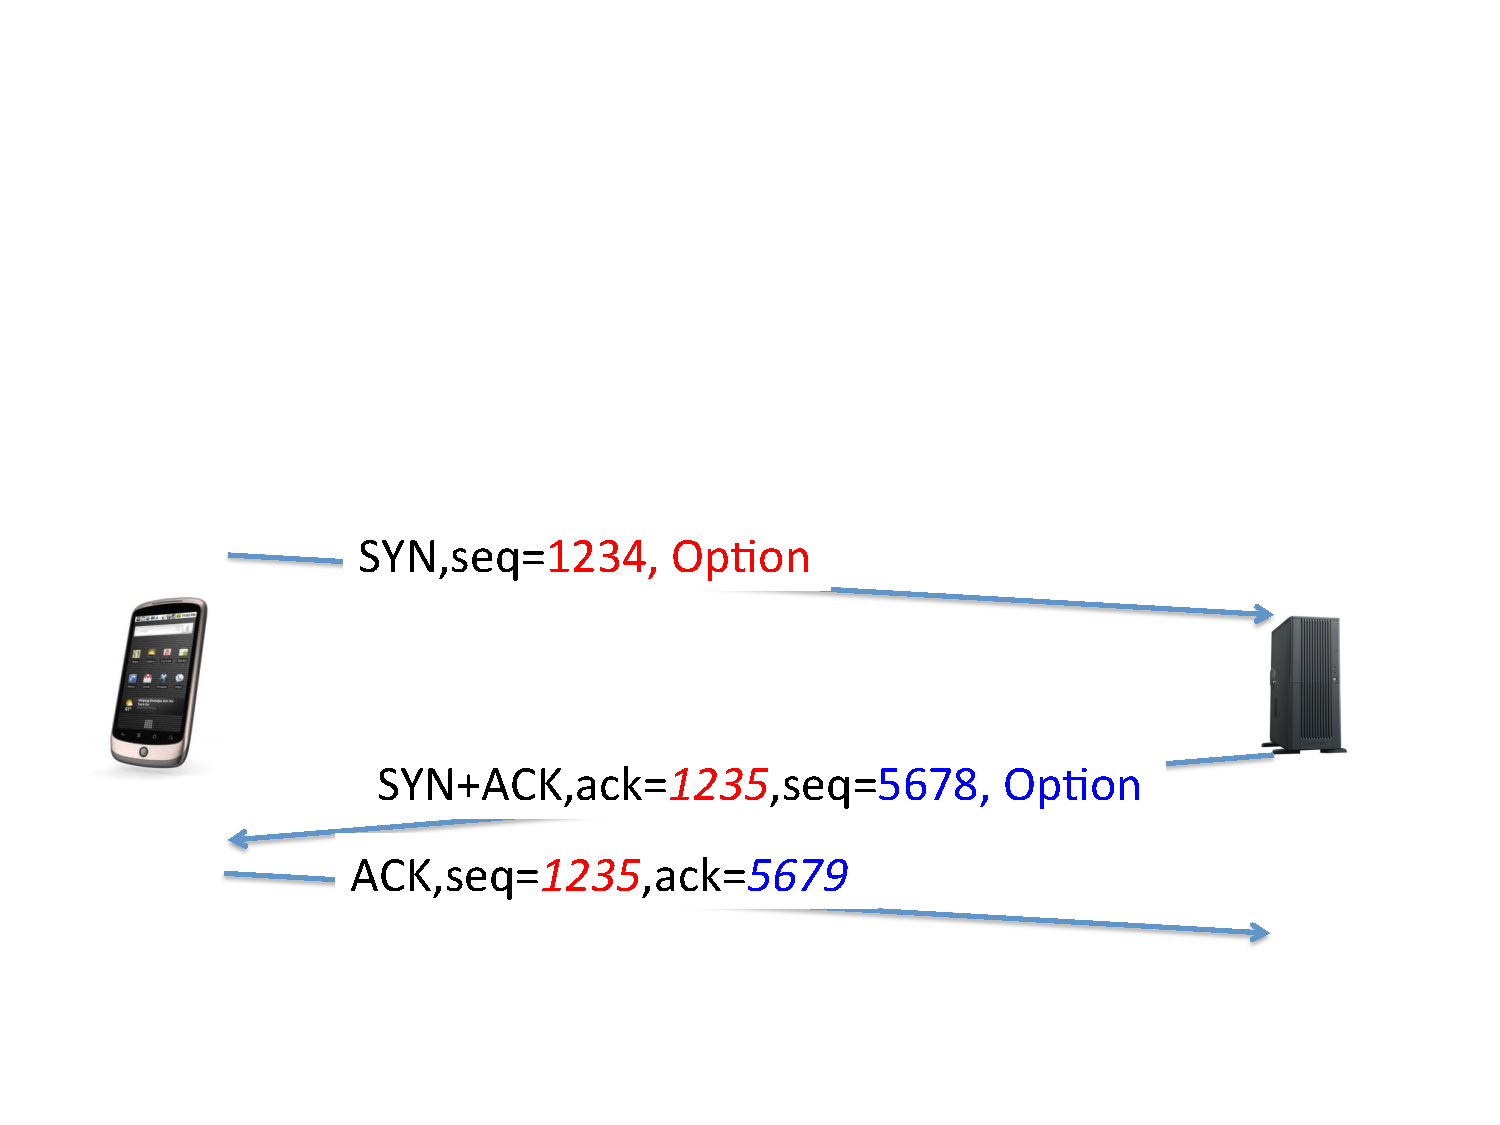
\includegraphics[width=0.8\textwidth]{figures/mptcp-ebook/Diapositive05.pdf}
\end{center}
\caption{TCP three-way handshake}\label{fig:tcp-establish}
\end{figure}


The duration of the three-way handshake is important for applications that exchange small amount of data such as requests for small web objects. It can become longer if losses occur because TCP can only rely on its retransmission timer to recover from the loss of a \texttt{SYN} or \texttt{SYN+ACK} segment. When a client sends a \texttt{SYN} segment to a server, it can only rely on the initial value of its retransmission timer to recover from losses\footnote{If the client has sent packets earlier to the same server, it might have stored some information from the previous connection \cite{rfc2140,Balakrishnan:1999:ICM:316188.316220} and use this information to bootstrap its initial timer. Recent Linux TCP/IP stacks preserve some state variables between connections.}. Most TCP/IP stacks have used an initial retransmission timer set to 3 seconds \cite{rfc1122}. This conservative value was chosen in the 1980s and confirmed in the early 2000s \cite{rfc2988}. However, this default implies that with many TCP/IP stacks, the loss of any of the first two segments of a three-way handshake will cause a delay of 3 seconds on a connection that may normally be shorter than that. Measurements conducted on large web farms showed that this initial timer had a severe impact on the performance perceived by the end users \cite{Chu_Tuning:2009}. This convinced the IETF to decrease the recommended initial value for the retransmission timer to 1 second \cite{rfc6298}. Some researchers proposed to decrease even more the value of the retransmission timer, notably in datacenter environments \cite{Vasudevan:2009:SEF:1592568.1592604}.

Another utilization of the three-way handshake is to negotiate options that are applicable for this connection. TCP was designed to be extensible. Although it does not carry a version field, in contrast with IP for example, TCP supports the utilization of options to both negotiate parameters and extend the protocol. 
TCP options in the \texttt{SYN} segment allow to negotiate the utilization of a particular TCP extension. To enable a particular extension, the client places the corresponding option inside the \texttt{SYN} segment. If the server replies with a similar option in the \texttt{SYN+ACK} segment, the extension is enabled. Otherwise, the extension is disabled on this particular connection. This is illustrated in figure~\ref{fig:tcp-establish}.


Each TCP option is encoded by using a Type-Length-Value (TLV) format, which enables a receiver to silently discard the options that it does not understand. Unfortunately, there is a limit to the maximum number of TCP options that can be placed inside the TCP header. This limit comes from the \texttt{Data Offset} field of the TCP header that indicates the position of the first byte of the payload measured as an integer number of four bytes word starting from the beginning of the TCP header. Since this field is encoded in four bits, the TCP header cannot be longer than 60 bytes, including all options. This size was considered to be large enough by the designers of the TCP protocol, but is becoming a severe limitation to the extensibility of TCP. 

A last point to note about the three-way handshake is that the first TCP implementations created state upon reception of a \texttt{SYN} segment. Many of these implementations also used a small queue to store the TCP connections that had received a \texttt{SYN} segment but not yet the third \texttt{ACK}. For a normal TCP connection, the delay between the reception of a \texttt{SYN} segment and the reception of the third \texttt{ACK} is equivalent to a round-trip-time, usually much less than a second. For this reason, most early TCP/IP implementations chose a small fixed size for this queue. Once the queue was full, these implementations dropped all incoming \texttt{SYN} segments. This fixed-sized queue was exploited by attackers to cause denial of service attacks. They sent a stream of spoofed \texttt{SYN} segment\footnote{An IP packet is said to be spoofed if it contains a source address which is different from the IP address of the sending host. Several techniques can be used by network operators to prevent such attacks \cite{rfc2827}, but measurements show that they are not always deployed \cite{Beverly:2009:UED:1644893.1644936}.} to a server. Once the queue was full, the server stopped accepting \texttt{SYN} segments from legitimate clients \cite{rfc4987}. To solve this problem, recent TCP/IP stacks try to avoid maintaining state upon reception of a \texttt{SYN} segment. This solution is often called \emph{syn cookies}. 

The principles behind \emph{syn cookies} are simple. To accept a TCP connection without maintaining state upon reception of the \texttt{SYN} segment, the server must be able to check the validity of the third \texttt{ACK} by using only the information stored inside this \texttt{ACK}. A simple way to do this is to compute the initial sequence number used by the server from a hash that includes the source and destination addresses and ports and some random secret known only by the server. The low order bits of this hash are then sent as the initial sequence number of the returned \texttt{SYN+ACK} segment. When the third \texttt{ACK} comes back, the server can check the validity of the acknowledgment number by recomputing its initial sequence number by using the same hash \cite{rfc4987}. Recent TCP/IP stacks use more complex techniques to deal notably with the options that are placed inside the \texttt{SYN} and need to be recovered from the information contained in the third \texttt{ACK} that usually does not contain any option.

At this stage, it is interesting to look at the connection establishment scheme used by the SCTP protocol \cite{rfc4960}. SCTP was designed more than two decades after TCP and thus has benefited from several of the lessons learned from the experience with TCP. A first difference between TCP and SCTP are the segments that these protocols use. The SCTP header format is both simpler and more extensible than the TCP header. 

The first four fields of the SCTP header (Source and Destination ports, Verification tag and Checksum) are present in all SCTP segments. The source and destination ports play the same role as in TCP. The verification tag is a random number chosen when the SCTP connection is created and placed in all subsequent segments. This verification tag is used to prevent some forms of packet spoofing attacks \cite{rfc4960}. This is an improvement compared to TCP where the validation of a received segment must be performed by checking the sequence numbers, acknowledgment numbers and other fields of the header \cite{Gont_TCPSecurity:2012}. The SCTP checksum is a 32 bits CRC that provides stronger error detection properties than the Internet checksum used by TCP \cite{Stone:2000:CTC:347059.347561}. Each SCTP segment can contain a variable number of chunks and there is no apriori limit to the number of chunks that appear inside a segment, except that a segment should not be longer than the maximum packet length of the underlying network layer.

The SCTP connection establishment uses several of these chunks to specify the values of some parameters that are exchanged. A detailed discussion of all these chunks is outside the scope of this document and may be found in \cite{rfc4960}. The SCTP four-way handshake uses four segments as shown in figure~\ref{fig:sctp-4way}. The first segment contains the \texttt{INIT} chunk. To establish an SCTP connection with a server, the client first creates some local state for this connection. The most important parameter of the \texttt{INIT} chunk is the \emph{Initiation tag}. This value is a random number that is used to identify the connection on the client host for its entire lifetime. This \emph{Initiation tag} is placed as the \emph{Verification tag} in all segments sent by the server. This is an important change compared to TCP where only the source and destination ports are used to identify a given connection. The \texttt{INIT} chunk may also contain the other addresses owned by the client. The server responds by sending an \texttt{INIT-ACK} chunk. This chunk also contains an \emph{Initiation tag} chosen by the server and a copy of the \emph{Initiation tag} chosen by the client. The \texttt{INIT} and \texttt{INIT-ACK} chunks also contain an initial sequence number. A key difference between TCP's three-way handshake and SCTP's four-way handshake is that an SCTP server does not create any state when receiving an \texttt{INIT} chunk. For this, the server places inside the \texttt{INIT-ACK} reply a \emph{State cookie} chunk. This \emph{State cookie} is an opaque block of data that contains information from the \texttt{INIT} and \texttt{INIT-ACK} chunks that the server would have had stored locally, some lifetime information and a signature. The format of the \emph{State cookie} is flexible and the server could in theory place almost any information inside this chunk. The only requirement is that the \emph{State cookie}  must be echoed back by the client to confirm the establishment of the connection. Upon reception of the \texttt{COOKIE-ECHO} chunk, the server verifies the signature of the \emph{State cookie}. The client may provide some user data and an initial sequence number inside the \texttt{COOKIE-ECHO} chunk. The server then responds with a \texttt{COOKIE-ACK} chunk that acknowledges the \texttt{COOKIE-ECHO} chunk. The SCTP connection between the client and the server is now established. This four-way handshake is both more secure and more flexible than the three-way handshake used by TCP. 

\begin{figure}
\begin{center}
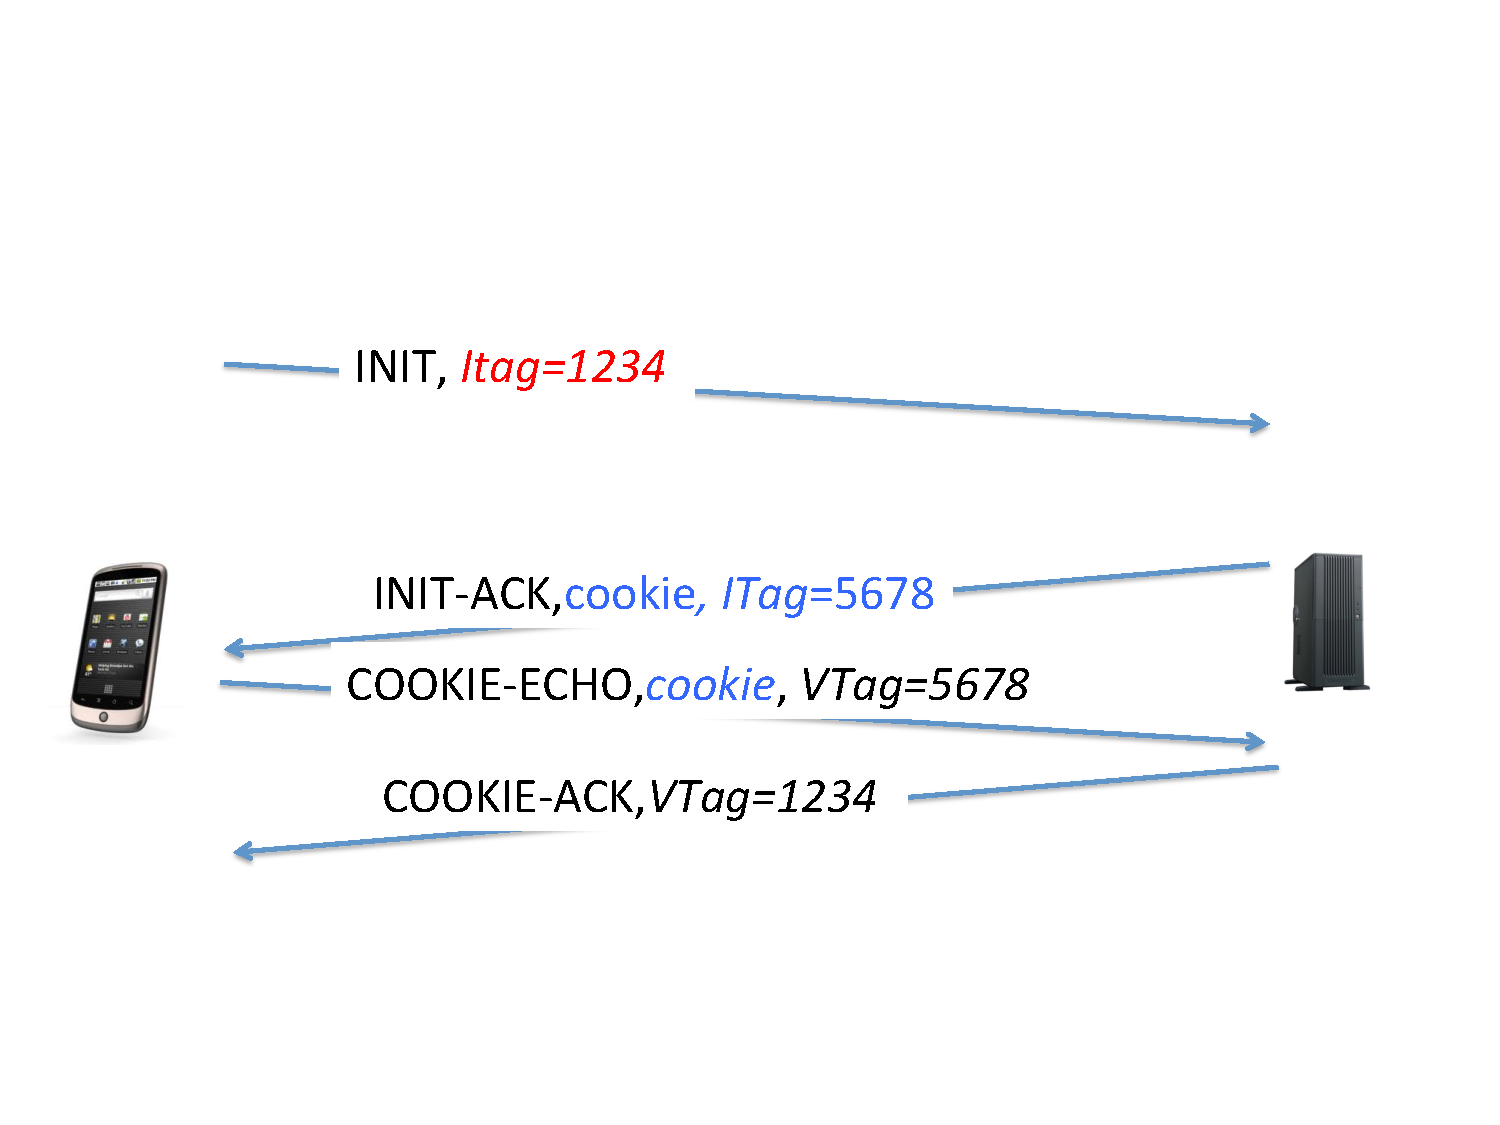
\includegraphics[width=0.8\textwidth]{figures/mptcp-ebook/Diapositive06.pdf}
\end{center}
\caption{The four-way handshake used by SCTP}\label{fig:sctp-4way}
\end{figure}


\subsubsection{Data transfer}

Before looking at the techniques that are used by transport protocols to transfer data, it is useful to look at their service models. TCP has the simplest service model. Once a TCP connection has been established, two bytestreams are available. The first bytestream allows the client to send data to the server and the second bytestream provides data transfer in the opposite direction. TCP guarantees the reliable delivery of the data during the lifetime of the TCP connection provided that it is gracefully released.

SCTP provides a slightly different service model \cite{rfc3286}. Once an SCTP connection has been established, the communicating hosts can access two or more message streams. A message stream is a stream of variable length messages. Each message is composed of an integer number of bytes. The connection-oriented service provided by SCTP preserves the message boundaries. This implies that if an application sends a message of \emph{N} bytes, the receiving application will also receive it as a single message of \emph{N} bytes. This is in contrast with TCP that only supports a bytestream. Furthermore, SCTP allows the applications to use multiple streams to exchange data. The number of streams that are supported on a given connection is negotiated during connection establishment. When multiple streams have been negotiated, each application can send data over any of these streams and SCTP will deliver the data from the different streams independently without any head-of-line blocking. 
%TCP provides some support for urgent data which could be considered as a restricted form of out-of-band capability. However, this part of the TCP specification has not been implemented in the same way on all TCP stacks \cite{rfc6093}.

While most usages of SCTP may assume an in-order delivery of the
data, SCTP supports unordered delivery of messages at the receiver. 
Another extension to SCTP \cite{rfc3758} supports partially-reliable delivery. With this
extension,  an SCTP sender can be instructed to ``expire'' data based on 
one of several events,
such as a timeout,
the sender can signal the SCTP receiver to move on without waiting for 
the ``expired'' data.
%a receiver may accept gaps inside the received data and
%still acknowledge the corresponding segments to the sender. 
This
partially reliable service could be useful to provide timed delivery
for example. With this service, there is an upper limit on the time
required to deliver a message to the receiver. If the
transport layer cannot deliver the data within the specified delay,
the data is discarded by the sender without causing any stall in the stream.

To provide a reliable delivery of the data, transport protocols rely on various mechanisms that have been well studied and discussed in the literature : sequence numbers, acknowledgments, windows, checksums and retransmission techniques. A detailed explanation of these techniques may be found in standard textbooks \cite{Bonaventure_CNP3:2012,ross2003computer,Fall_TCP:2011}. We assume that the reader is familiar with them and discuss only some recent changes. 


TCP tries to pack as much data as possible inside each segment \cite{rfc793}. Recent TCP stacks combine this technique with Path MTU discovery to detect the MTU to be used over a given path \cite{rfc4821}. SCTP uses a more complex but also more flexible strategy to build its segments. It also relies on Path MTU Discovery to detect the MTU on each path. SCTP then places various chunks inside each segment. The control chunks, that are required for the correct operation of the protocol, are placed first. Data chunks are then added. SCTP can split a message in several chunks before transmission and also the bundling of different data chunks inside the same segment.

% packet nagle in TCP, bundling in SCTP for lagre and small

Acknowledgments allow the receiver to inform the sender of the correct reception of data. TCP initially relied exclusively on cumulative acknowledgments. Each TCP segment contains an acknowledgment number that indicates the next sequence number that is expected by the receiver. Selective acknowledgments were added later as an extension to TCP \cite{rfc2018}. A selective acknowledgment can be sent by a receiver when there are gaps in the received data. A selective acknowledgment is simply a sequence of pairs of sequence numbers, each pair indicating the beginning and the end of a received block of data. SCTP also supports cumulative and selective acknowledgments. Selective acknowledgments are an integral part of SCTP and not an extension which is negotiated at the beginning of the connection. In SCTP, selective acknowledgments are encoded as a control chunk that may be placed inside any segment. In TCP, selective acknowledgments are encoded as TCP options. Unfortunately, given the utilization of the TCP options (notably the timestamp option \cite{rfc1323}) and the limited space for options inside a TCP segment, a TCP segment cannot report more than three blocks of data. This adds some complexity to the handling and utilization of selective acknowledgments by TCP.

Current TCP and SCTP stacks try to detect segment losses as quickly as possible. For this, they implement various heuristics that allow to retransmit a segment once several duplicate acknowledgments have been received \cite{Fall_TCP:2011}. Selective acknowledgment also aid to improve the retransmission heuristics. If these heuristics fail, both protocols rely on a retransmission timer whose value is fixed in function of the round-trip time measured over the connection \cite{rfc6298}.

Last but not least, the transport protocols on the Internet perform congestion control. The original TCP congestion control scheme was proposed in \cite{Jacobson_congestion:88}. Since then, it has evolved and various congestion control schemes have been proposed. Although the IETF recommends a single congestion control scheme \cite{rfc5681}, recent TCP stacks support different congestion control schemes and some allow the user to select the preferred one. A detailed discussion of the TCP congestion control schemes may be found in \cite{Afanasyev_Congestion:2012}. SCTP's congestion control scheme is largely similar to TCP's congestion control scheme. 

Additional details about recent advances in SCTP may be found in \cite{Budzisz_Taxonomy:2012}. \cite{rfc4614} lists recent IETF documents that are relevant for TCP. \cite{Fall_TCP:2011} contains a detailed explanation of some of the recent changes to the TCP/IP protocol stack.


\subsubsection{Connection release}

\begin{figure}
\begin{center}
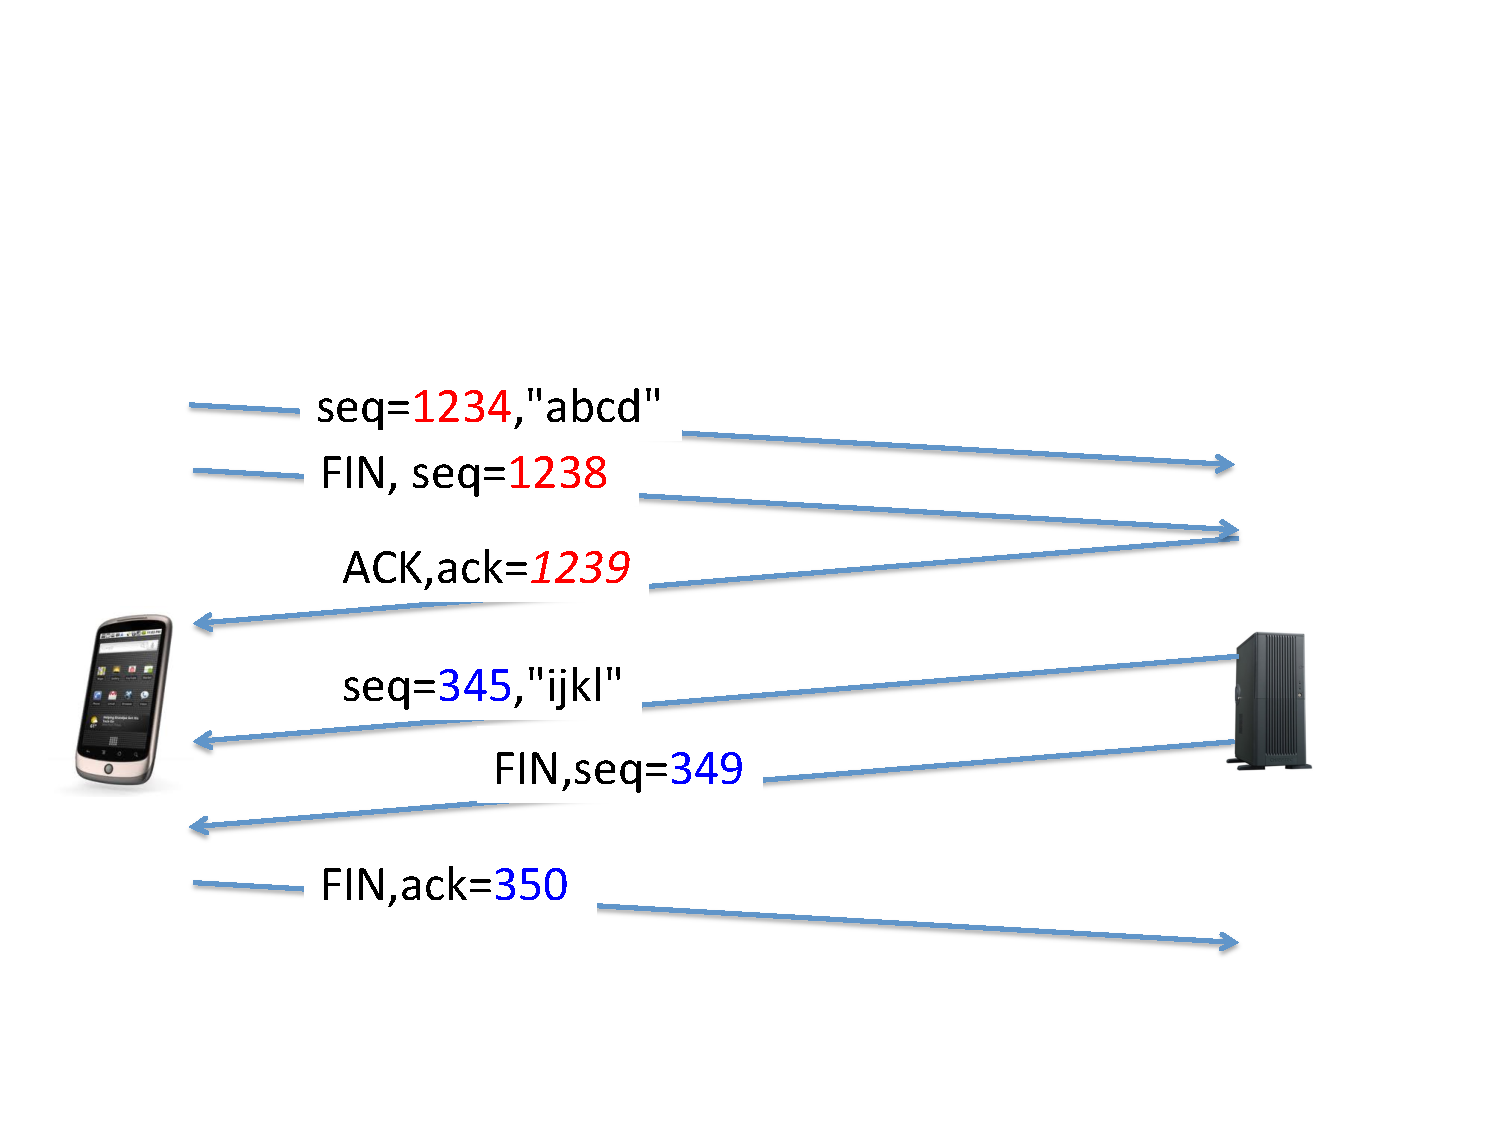
\includegraphics[width=0.8\textwidth]{figures/mptcp-ebook/Diapositive08.pdf}
\end{center}
\caption{The four-way handshake used to close a TCP connection}\label{fig:tcp-fin}
\end{figure}

This phase occurs when either both hosts have exchanged all the required data or when one host needs to stop the connection for any reason (application request, lack of resources, \ldots). TCP supports two mechanisms to release a connection. The main one is the four-way handshake. This handshake uses the \texttt{FIN} flag in the TCP header. Each host can release its own direction of data transfer. When the application wishes to gracefully close a connection, it requests the TCP entity to send a \texttt{FIN} segment. This segment marks the end of the data transfer in the outgoing direction and the sequence number that corresponds to the \texttt{FIN} flag (which consumes one sequence number) is the last one to be sent over this connection. The outgoing stream is closed as soon as the sequence number corresponding to the \texttt{FIN} flag is acknowledged. The remote TCP entity can use the same technique to close the other direction \cite{rfc793}. This graceful connection release has one advantage and one drawback. On the positive side, TCP provides a reliable delivery of all the data provided that the connection is gracefully closed. On the negative side, the utilization of the graceful release forces the TCP entity that sent the last segment on a given connection to maintain state for some time. On busy servers, a large number of connections can remain for a long time \cite{Faber_TimeWait:1999}. To avoid maintaining such state after a connection has been closed, web servers and some browsers send a \texttt{RST} segment to abruptly close TCP connections. In this case, the underlying TCP connection is closed once all the data has been transferred. This is faster, but there is no guarantee about the reliable delivery of the data. 


SCTP uses a different approach to terminante connections. When an application requests a shutdown of a connection, SCTP performs a three-way handshake. This handshake uses the \texttt{SHUTDOWN}, \texttt{SHUTDOWN-ACK} and \texttt{SHUTDOWN-COMPLETE} chunks. The \texttt{SHUTDOWN} chunk is sent once all outgoing data has been acknowledged. It contains the last cumulative sequence number. Upon reception of a \texttt{SHUTDOWN} chunk, an SCTP entity informs its application that it cannot accept anymore data over this connection. It then ensures that all outstanding data have been delivered correctly. At that point, it sends a \texttt{SHUTDOWN-ACK} to confirm the reception of the \texttt{SHUTDOWN} segment. The three-way handshake completes with the transmission of the \texttt{SHUTDOWN-COMPLETE} chunk \cite{rfc4960}.

\begin{figure}
\begin{center}
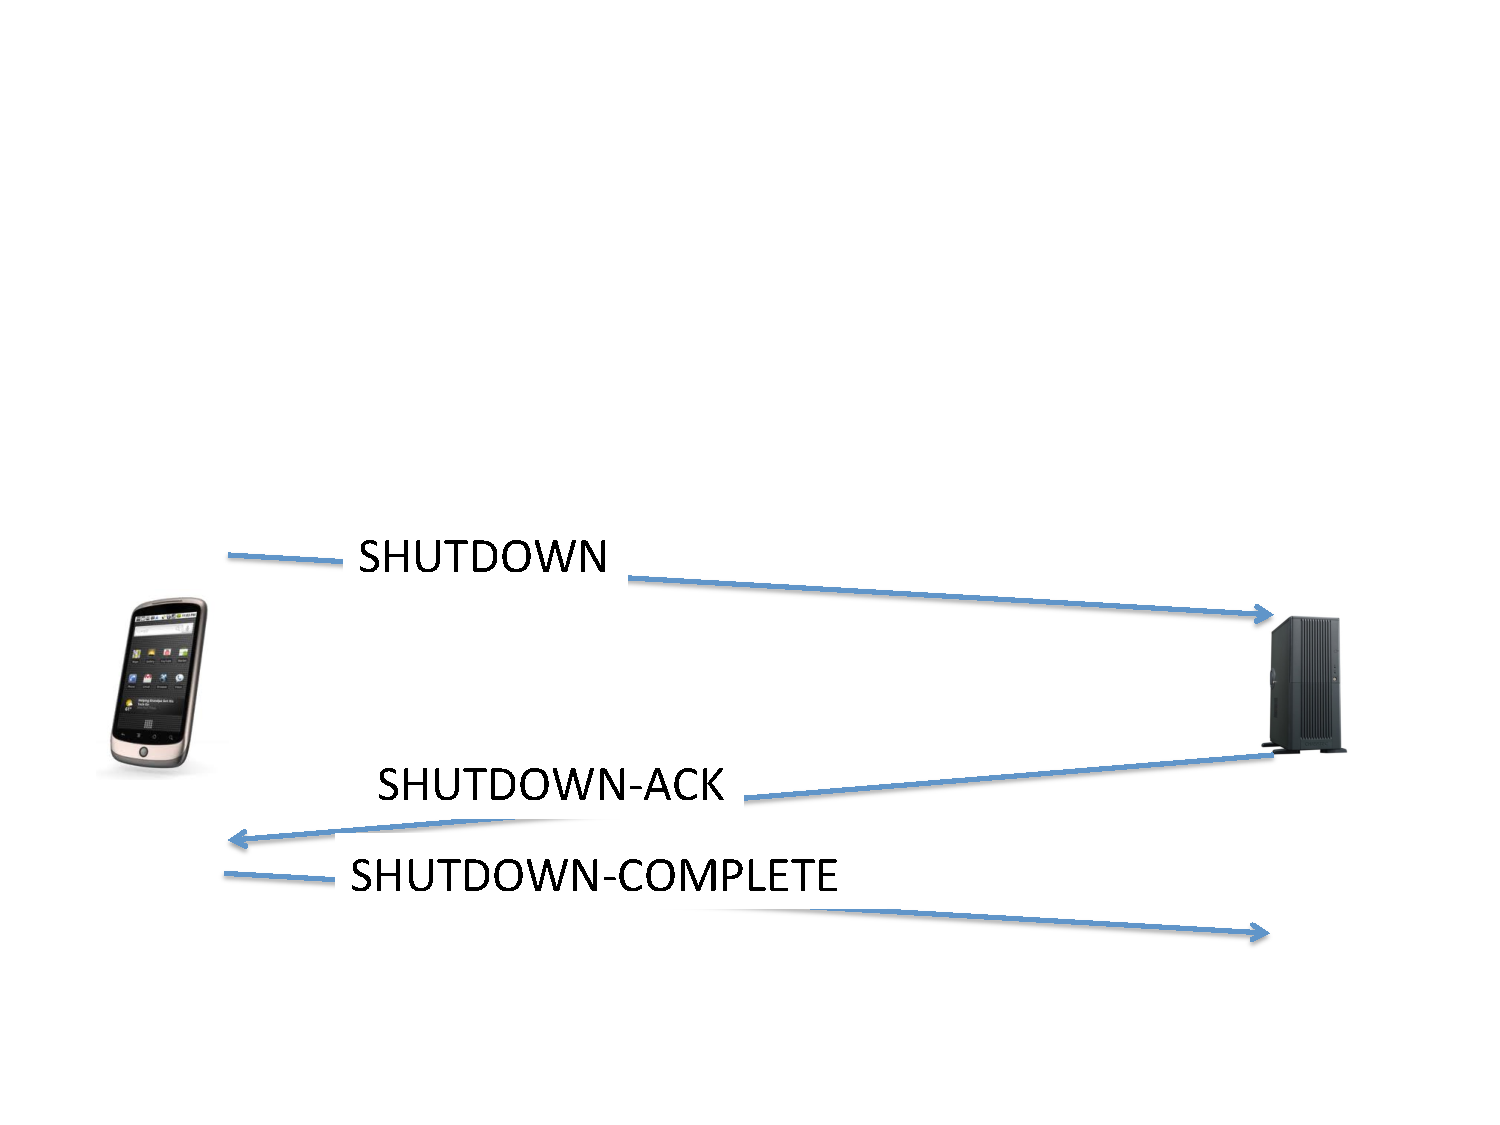
\includegraphics[width=0.8\textwidth]{figures/mptcp-ebook/Diapositive11.pdf}
\end{center}
\caption{The three-way handshake used to close an SCTP connection}\label{fig:sctp-close}
\end{figure}

SCTP also provides the equivalent to TCP's \texttt{RST} segment. The \texttt{ABORT} chunk can be used to refuse a connection, react to the reception of an invalid segment or immediately close a connection (e.g. due to lack of resources).

\subsection{Providing the request-response service}
%---------------------------------------------------

The request-response service has been a popular service since the 1980s.  At that time, many request-response applications were built above the connectionless service, typically UDP \cite{Birrell_RPC:1984}. A request-response application is very simple. The client sends a request to a server and blocks waiting for the response. The server processes the request and returns a response to the client. This paradigm is often called Remote Procedure Call (RPC) since often the client calls a procedure running on the server. 

The first implementations of RPC relied almost exclusively on UDP to transmit the request and responses. In this case, the size of the requests and responses was often restricted to one MTU. In the 1980s and the beginning of the 1990s, UDP was a suitable protocol to transport RPCs because they were mainly used in Ethernet LANs. Few users were considering the utilization of RPC over the WAN. In such networks, CSMA/CD regulated the access to the LAN and there were almost no losses. Over the years, the introduction of Ethernet switches has both allowed Ethernet networks to grow in size but also implied a growing number of packet losses. Unfortunately, RPC running over UDP does not deal efficiently with packet losses because many implementation use large timeouts to recover for packet losses. TCP could deal with losses, but it was considered to be too costly for request-response applications. Before sending a request, the client must first initiate the connection. This requires a three-way handshake and thus ``wastes'' one round-trip-time. Then, TCP can transfer the request and receive the response over the established connection. Eventually, it performs a graceful shutdown of the connection. This connection release requires the exchange of four (small) segments, but also forces the client to remain in the \texttt{TIME\_WAIT} state for a duration of 240 seconds, which limits the number of connections (and thus RPCs) that it can establish with a given server.

TCP for Transactions or T/TCP \cite{rfc1644} was a first attempt to enable TCP to better support request/response applications. T/TCP solved the above problem by using three TCP options. These options were mainly used to allow each host to maintain an additional state variable, Connection Count (CC) that is incremented by one for every connection. This state variable is sent in the \texttt{SYN} segment and cached by the server. If a \texttt{SYN} received from a client contains a CC that is larger than the cached one, the new connection is immediately established and data can be exchanged directly (already in the \texttt{SYN}). Otherwise, a normal three-way handshake is used. The use of this state variable allowed T/TCP to reduce the duration of the \texttt{TIME\_WAIT} state. T/TCP used \texttt{SYN} and \texttt{FIN} flags in the segment sent by the client and returned by the server, which led to a two segment connection, the best solution from a delay viewpoint for RPC applications. Unfortunately, T/TCP was vulnerable to spoofing attacks \cite{deVivo_TTCP:1999}. An attacker could observe the Connection Count by capturing packets. Since the server only checked that the value of the CC state variable contained in a \texttt{SYN} segment was higher than the cached one, it was easy to inject new segments. Due to this security problem, T/TCP is now deprecated.


Improving the performance of TCP for request/response applications continued to be an objective for many researchers. However, recently the focus of the optimizations moved from the LANs that were typical for RPC applications to the global Internet. The motivation for several of the recent changes to the TCP protocol was the perceived performance of TCP with web search applications \cite{Chu_Tuning:2009}. A typical web search is also a very short TCP connection during which a small HTTP request and a small HTTP response are exchanged. A first change to TCP was the increase of the initial congestion window \cite{Chu_increasing:2013}. For many years, TCP used an initial window between 2 and 4 segments \cite{rfc3390}. This was smaller than the typical HTTP response from a web search engine \cite{Chu_Tuning:2009}. Recent TCP stacks use an initial congestion window of 10 segments \cite{Chu_increasing:2013}.

\begin{figure}
\begin{center}
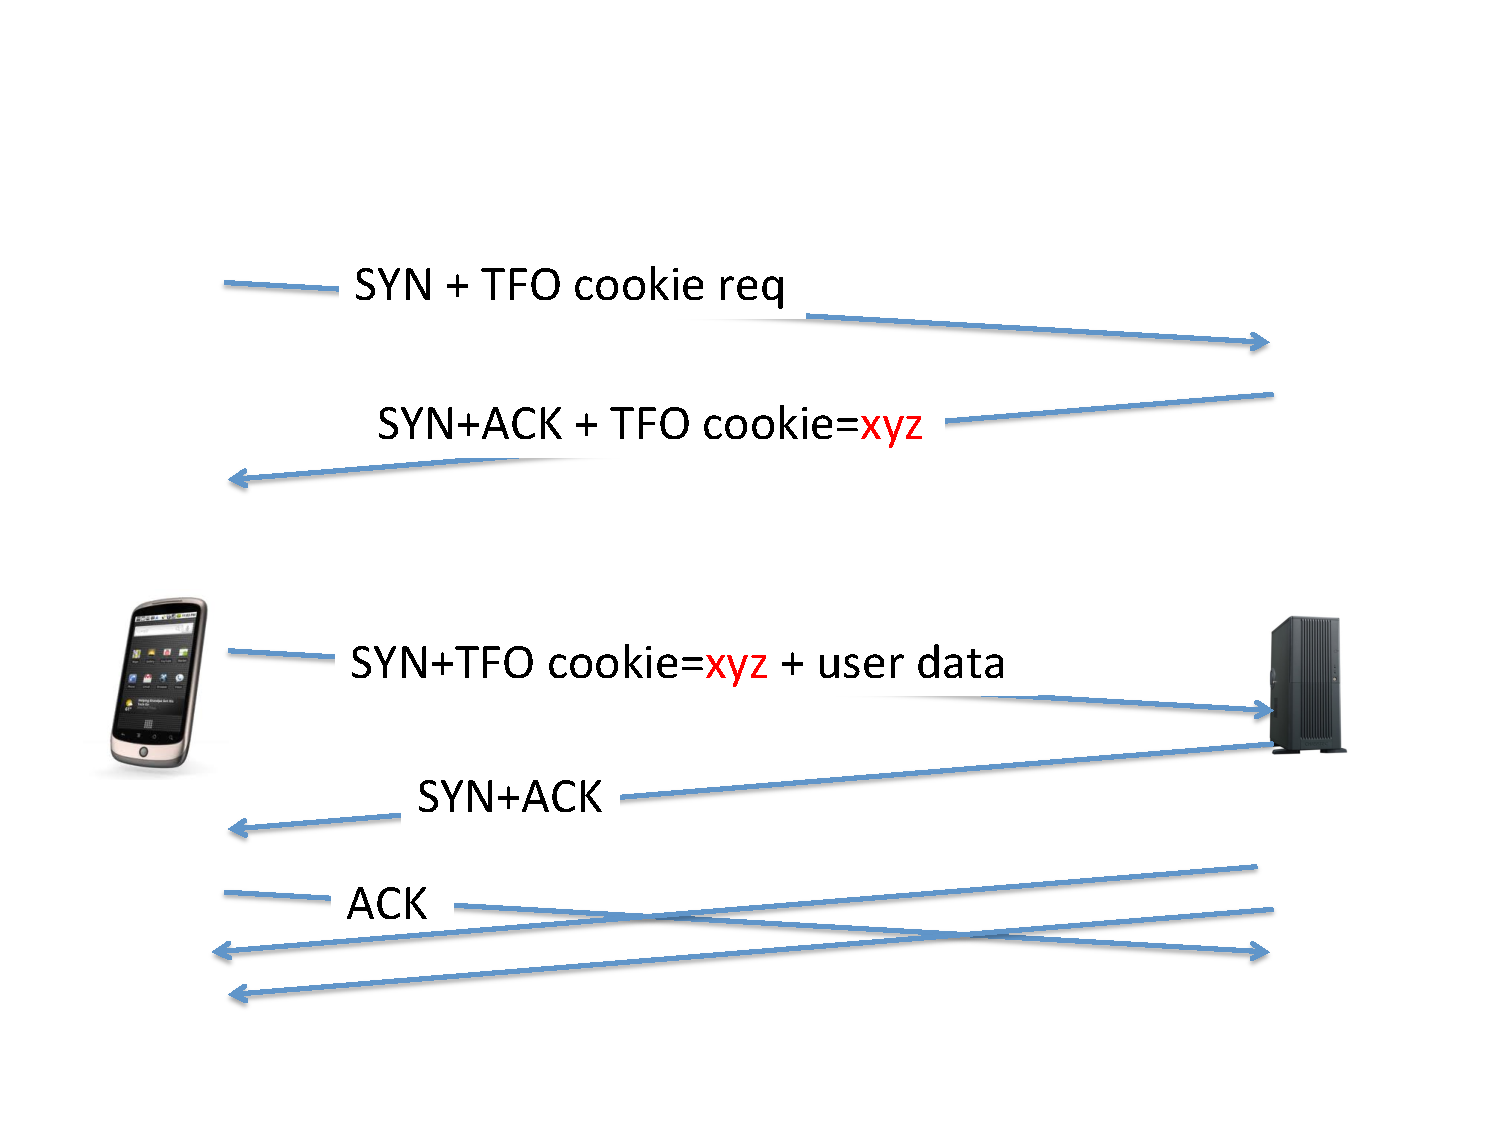
\includegraphics[width=0.8\textwidth]{figures/mptcp-ebook/Diapositive12.pdf}
\end{center}
\caption{TCP fast open}\label{fig:tcp-fastopen}
\end{figure}


Another change that has been motivated by web search applications is the TCP Fast Open (TFO) extension \cite{radhakrishnan2011tcp}. This extension can be considered as a replacement for T/TCP. TCP fast open also enables a client to send data inside the \texttt{SYN} segment. TCP fast open relies on state sharing between the client and the server, but the state is more secure than the simple counter used by T/TCP. To enable the utilization of TCP fast open, the client must first obtain a \emph{cookie} from the server. This is done by sending a \texttt{SYN} segment with the TFO cookie request option. The server then generates a secure cookie by encrypting the IP address of the client with a local secret \cite{radhakrishnan2011tcp}. The encrypted information is returned inside a TFO cookie option in the \texttt{SYN+ACK} segment. The client caches the cookie and associates it with the server's IP address. The subsequent connections initiated by the client will benefit from TCP fast open. The client includes the cached cookie and optional data inside its \texttt{SYN} segment. The server can validate the segment by decrypting its cookie. If the cookie is valid, the server acknowledges the \texttt{SYN} and the data that it contains. Otherwise, the optional data is ignored and a normal TCP three-way handshake is used. This is illustrated in figure~\ref{fig:tcp-fastopen}.


